\documentclass[a4paper,11pt]{report}

\usepackage{fullpage}

\usepackage{amsmath}
\usepackage{bussproofs}
\usepackage{mathpartir}
\usepackage{prooftrees}
\usepackage{color}
\usepackage{hyperref}
\usepackage{placeins}
\usepackage{tabularx}
\usepackage[normalem]{ulem}
\useunder{\uline}{\ul}{}


% for finite state automata
\usepackage{tikz}
\usetikzlibrary{automata,positioning}

%%%%%%%%%%%%%%%%%%%%%%%%%%%%%%%%%%%%%%%%%%%%%%%%%%%%%%%%%
% Minted
%%%%%%%%%%%%%%%%%%%%%%%%%%%%%%%%%%%%%%%%%%%%%%%%%%%%%%%%%

\usepackage[cache=false]{minted}

%%%%%%%%%% C
\newmintinline{c}{
  fontsize=\small,
  breaklines=true
}

\newminted{c}{
  frame=single,
  framesep=2mm,
  fontsize=\scriptsize,
  mathescape
}

\newminted[ccodeline]{c}{
  frame=single,
  framesep=2mm,
  fontsize=\scriptsize,
  mathescape,
  linenos
}

%%%%%%%%% CMAKE
\newminted{cmake}{
  frame=single,
  framesep=2mm,
  fontsize=\scriptsize,
  mathescape,
  linenos,
  breaklines=true
}

% End minted
%%%%%%%%%%%%%%%%%%%%%%%%%%%%%%%%%%%%%%%%%%%%%%%%%%%%%%%%%


\author{Sylvain Julmy}
\date{\today}

\setlength{\parindent}{0pt}

\begin{document}

\begin{center}
  \Large{
    Operating Systems\\
    Spring 2018
  }
  
  \noindent\makebox[\linewidth]{\rule{\linewidth}{0.4pt}}
  S09
  \noindent\makebox[\linewidth]{\rule{\linewidth}{0.4pt}}
  \begin{flushleft}
    Professor : Philippe Cudré-Mauroux

    Assistant : Ines Arous
  \end{flushleft}
  
  \noindent\makebox[\linewidth]{\rule{\linewidth}{0.4pt}}

  Submitted by Sylvain Julmy
  
  \noindent\makebox[\linewidth]{\rule{\textwidth}{1pt}}
\end{center}

\section*{Exercise 2}

\subsection*{\texttt{a)}}

An i-node is a data structure that a filesystem object like a file or a
directory. Each inode stores the attributes and disk block location(s) of the
object's data. Filesystem object attributes may include metadata (times of last
change, access, modification), as well as owner and permission data.

The i-node is associated with a filename, give a filename the directory knows
where to find the i-node and the i-node knows where to find the file on the disk.

\subsection*{\texttt{b)}}

There are $3$ i-nodes : $usr$, $src$ and $kernels$ and $4$ directory block :
$/$, $usr$, $src$ and $kernels$. So there are $4 + 3 = 7$ total disk access.

\section*{Exercise 3}

\verb+rename+ in the current directory only changes the filename in the
directory entry. \verb+rename+ in a different directory add an entry to the new
directory which point on the same i-node and remove the entry in the old one.

\verb+cp+ just create a new i-node and \verb+rm+ decreases the reference counter
of the i-node.

\section*{Exercise 4}

A symbolic link is just a file which contains the path of the targeted file and
a hard link is a filename which point to the same i-node.

\subsection*{\texttt{a)}}

Advantages of hard links :
\begin{itemize}
\item The link is working even if a file is removed.
\item Moving the link on the same disk does not break the link.
\end{itemize}

Advantages of symbolic links :
\begin{itemize}
\item Can point to any file where hard links can only point on the same disk
\end{itemize}

\subsection*{\texttt{b)}}

A Windows shortcute is a symbolic link.

\subsection*{\texttt{c)}}

An OSX's alias is a symbolic link.

\section*{Exercise 5}

\paragraph{What are the i-node values of file1.txt and file2.txt? Are they the
  same or different?}

The i-node values are the same like in figure \ref{fig:ex5-a}.

\begin{figure}[h]
  \centering
  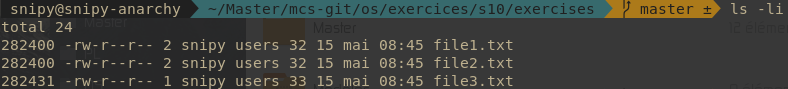
\includegraphics[width=0.99\textwidth]{figures/ex5-a}
  \caption{\label{fig:ex5-a} The i-node value of the file and the hard link is the same.}
\end{figure}

\paragraph{Do the two files have the same or different contents ?}

Both files owns the same content as seen in figure \ref{fig:ex5-b}.

\begin{figure}[h]
  \centering
  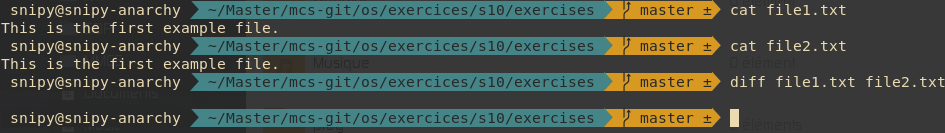
\includegraphics[width=0.99\textwidth]{figures/ex5-b}
  \caption{\label{fig:ex5-b} The content of both file is identical.}
\end{figure}

\paragraph{Are the cont ents of file1.txt and file2.txt the same or different?}

The contents remains the same for both file as seen in figure \ref{fig:ex5-c}

\begin{figure}[h]
  \centering
  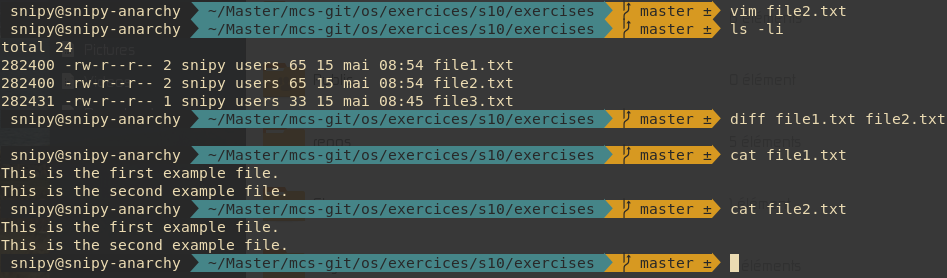
\includegraphics[width=0.99\textwidth]{figures/ex5-c}
  \caption{\label{fig:ex5-c} The content of both file is identical even after
    modifiying the content of the hard link.}
\end{figure}

\paragraph{Does file2.txt still exist as well ?}

After removing the file, the hard link still exists as in
figure~\ref{fig:ex5-d}.

\begin{figure}[h]
  \centering
  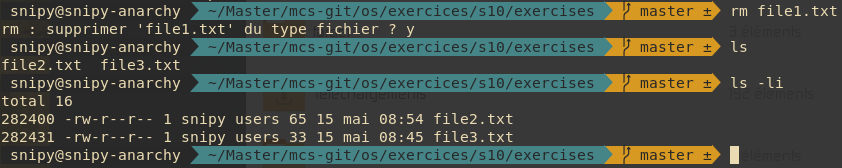
\includegraphics[width=0.99\textwidth]{figures/ex5-d}
  \caption{\label{fig:ex5-d} The hard link still exists after removing the real file.}
\end{figure}

\paragraph{What system call is used for removing file2.txt ?}

As seen in figure~\ref{fig:ex5-e}, there are a lot of different system call
used in order to remove a file.

\begin{figure}[h]
  \centering
  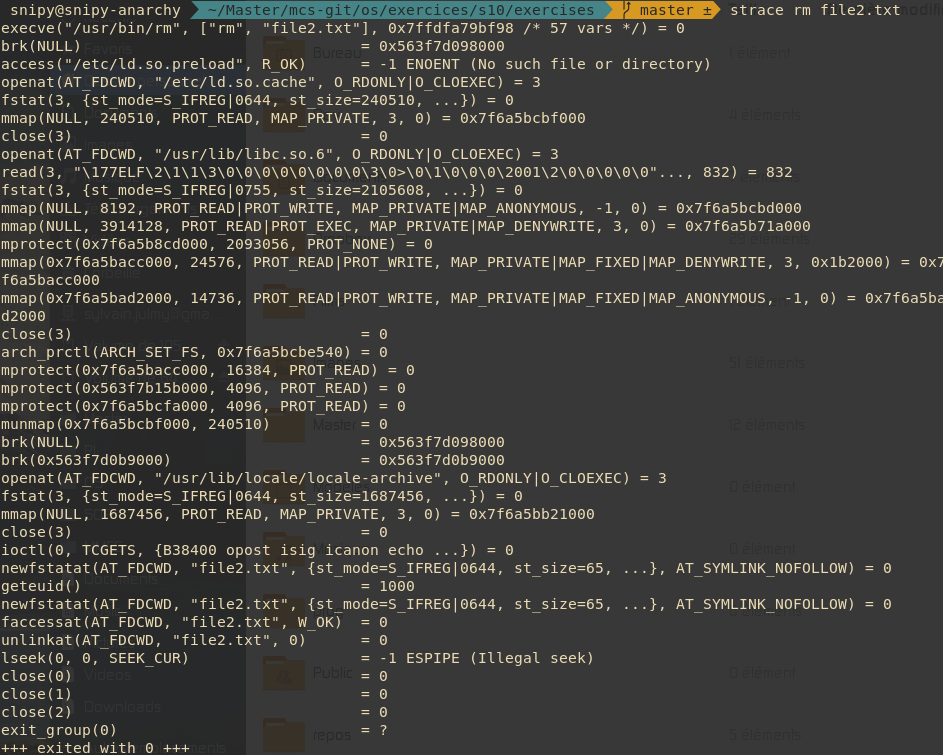
\includegraphics[width=0.99\textwidth]{figures/ex5-e}
  \caption{\label{fig:ex5-e} Output of the strace command when removing a hard link.}
\end{figure}

System call used by rm (not all, only the most impactfull) :

\begin{itemize}
\item \verb+mmap+ : establish a mapping between an address space of a process
  and a memory object.
\item \verb+close+ and \verb+read+ : close or read from a channel.
\item \verb+brk+ : modify the data segment size.
\item \verb+unlinkat+ : delete a name and possibly the file it refers to.
\end{itemize}

\end{document}
